\documentclass{article}
\usepackage[preprint,nonatbib]{neurips_2024}
\makeatletter
\renewcommand{\@noticestring}{Rutgers University, Massive Data Mining course project. Report version 6.}
\makeatother
\usepackage[T1]{fontenc}
\usepackage{amsmath,booktabs,graphicx}
\usepackage{placeins}
\usepackage[hidelinks]{hyperref}
\title{AdaRetrieve: Sequential Retrieval and Reranking\\under Latency Budgets}
\author{Anuj Bohra \qquad Krisha Borana \qquad Dongquan Yang\\Rutgers University, New Brunswick\\Massive Data Mining}
\hypersetup{pdftitle={AdaRetrieve: Sequential Retrieval and Reranking under Latency Budgets},pdfauthor={Anuj Bohra, Krisha Borana and Dongquan Yang}}
\newcommand{\datatable}[1]{\begingroup\setlength{\tabcolsep}{4pt}\input{#1-table}\endgroup}
\newcommand{\widetable}[1]{\begingroup\setlength{\tabcolsep}{2.6pt}\input{#1-table}\endgroup}
\newcommand{\MatchedNTight}{0.0080}
\newcommand{\MatchedUTight}{0.0066}
\newcommand{\MatchedMsTight}{0.21}
\newcommand{\MatchedNMiddle}{0.0089}
\newcommand{\MatchedUMiddle}{0.0086}
\newcommand{\MatchedMsMiddle}{0.26}
\newcommand{\MatchedNLoose}{0.0080}
\newcommand{\MatchedULoose}{0.0078}
\newcommand{\MatchedMsLoose}{0.27}
\newcommand{\MedianCount}{528}
\newcommand{\MedianRate}{81.5\%}
\newcommand{\MedianN}{0.3332}
\newcommand{\MedianU}{0.2245}
\newcommand{\NinetyCount}{446}
\newcommand{\NinetyRate}{68.8\%}
\newcommand{\NinetyN}{0.3147}
\newcommand{\NinetyU}{0.2310}
\newcommand{\TailCount}{355}
\newcommand{\TailRate}{54.8\%}
\newcommand{\TailN}{0.3035}
\newcommand{\TailU}{0.2394}
\newcommand{\NinetyLoss}{0.0185}
\newcommand{\NinetyGain}{0.0065}
\newcommand{\NinetyPoints}{12.7}
\newcommand{\TailLoss}{0.0297}
\newcommand{\TailGain}{0.0149}
\newcommand{\TailPoints}{26.7}
\newcommand{\LongSciFact}{0.0478}
\newcommand{\LongNFCorpus}{0.0083}
\newcommand{\LongFiQA}{0.0057}
\newcommand{\TightForks}{529}
\newcommand{\TightMatchedOver}{514}

\begin{document}
\maketitle
\begin{abstract}
Can a single intermediate routing decision improve latency-bounded retrieval enough to justify its cost? Across three leave-one-domain-out BEIR folds (1,271 queries), the original end-to-end runs showed that giving a source-trained one-shot router one revision after dense retrieval raised equal-domain macro NDCG@10 by 0.0080--0.0089 and utility by 0.0079--0.0087. Two additional T4 runs isolate this decision and diagnose its bottlenecks without target tuning. Under matched-prefix execution, revision raised macro NDCG@10 by \MatchedNTight{}--\MatchedNMiddle{} and measured utility by \MatchedUTight{}--\MatchedUMiddle{} over one-shot routing, yet utility intervals against fixed reciprocal rank fusion (RRF) crossed zero at every budget. MiniLM-L6 improved NDCG@10 over TinyBERT and RRF and incurred substantial latency. In a separate diagnostic run, p95 source-domain admission at FiQA's 14 ms budget lowered overruns from \MedianRate{} to \TailRate{} relative to p50, at a cost of \TailLoss{} NDCG@10, while 384-token reranking raised NDCG@10 on SciFact and NFCorpus but improved middle-budget utility only on SciFact. These results remain exploratory on previously studied collections.

\end{abstract}

\section{Introduction}
A query whose lexical matches already answer it can finish after BM25. A query whose relevant documents use different terminology may benefit from a dense retrieval stage, even when that stage pays off only after fusion or reranking. Choosing a full path at the start keeps routing cheap. Choosing each action after seeing a new ranking gives the system more evidence, but the time spent acting and deciding also counts against the deadline. We compare these choices on a collection excluded from training, then test whether a single intermediate decision captures enough of the benefit to justify its cost.

\section{Related work}
BM25 ranks documents by lexical evidence \cite{bm25}. Reciprocal rank fusion combines the positions assigned by several retrievers \cite{rrf}, and a BERT cross-encoder can rescore the resulting query--document pairs \cite{bert}. Meng et al.\ \cite{trunc} study how far to truncate a retrieved list before reranking. Here the policy can also change which candidates enter the list and can stop before reranking. BEIR \cite{beir} supplies heterogeneous retrieval tasks on which to test whether those decisions transfer to another collection.

\section{Method}
\subsection{Actions and the serving budget}
Each adaptive query starts with up to 20 BM25 candidates. The policy can expand lexical retrieval to return up to 64 candidates, retrieve 20 dense candidates and expand to 64, fuse the lists using reciprocal rank fusion (RRF, k = 60), rerank the top 8 and then up to 24 documents, or stop. Extending reranking scores only previously unscored candidates. A gradient-boosted model with 40 depth-three trees selects each sequential action from query features, score statistics, rank overlap and change, and remaining budget.

The target utility for query $q$ with elapsed time $t_q$ and budget $B$ is
\begin{equation}
 U_q=\operatorname{NDCG@10}_q-0.035\,t_q/B-0.30\max(0,t_q/B-1).
 \label{eq:u}
\end{equation}
We compute $U_q$ from the returned ranking and measured wall time before averaging across queries and domains. The execution guard admits the next action only if its estimated cost fits within the remaining budget. Runtime variation can still produce an overrun.

\subsection{Learning from a finite-action oracle}
At each legal prefix the training oracle assigns Stop the utility of the current ranking. For any feasible continuation it assigns the largest terminal utility reachable from that child. This credits a retrieval step that helps only after a later fusion or reranking step. The cost estimates are frozen medians from the source domains. Pruning infeasible children keeps every enumerated state within budget, so the overrun term in Equation~\ref{eq:u} is zero throughout the training table. At evaluation the same term charges each observed overrun.

Both policies can use the same 30 terminal paths. The sequential policy observes intermediate rankings, while the one-shot policy chooses a path immediately after the initial BM25 ranking. The old full-grid router never split on path ID, causing every score to tie so argmax invariably picked Stop. The revised router fits a ridge regression for each path using its paired NDCG@10 gain over Stop. Six initial query and BM25 features determine the predicted gain, and the router subtracts the path's profiled time charge. The runtime guard can end a chosen path early. On source validation, it selected three to seven distinct paths per fold and budget and beat the best constant path in seven of nine settings under profiled costs.

\subsection{One optional decision after dense retrieval}
The one-shot and one-revision policies share the same root router and BM25 reuse. Their initial paths may differ because each timed run selects its default path based on its own elapsed time. Both fetch up to 64 BM25 candidates once, expose up to 20 until expansion, and use the same source-calibrated lexical costs. After a planned dense top-20 retrieval, a ridge model predicts suffix gains from scores and rank agreement. The router may switch once, including to Stop, if a feasible suffix improves predicted utility over the feasible default continuation by more than the frozen threshold. It never forces a dense probe.

\section{Experiments}
\subsection{Transfer design and evaluation}
Five T4 sessions comprise the broad benchmark, the root-only comparison, the BM25 reuse and revision comparison, a matched-prefix and reranker comparison, and a deadline, depth and truncation study. Timings cover query retrieval, feature computation, policy decisions, neural inference and the return of results to the CPU. All treatment contrasts use measurements from the same session.

Each training fold uses 384 queries from each source domain. Each source contributes a further 96 validation queries. FiQA and NFCorpus supply official development splits. SciFact reserves 15\% of its training pool for validation. The three target test sets contain 300 SciFact, 323 NFCorpus and 648 FiQA queries. The tight, middle and loose budgets are 17/37/68 ms for SciFact and NFCorpus and 14/30/56 ms for FiQA. We give each test domain equal weight. The T4 runs use the frozen multi-qa-MiniLM-L6-cos-v1 encoder, exact FAISS inner-product search and the ms-marco-TinyBERT-L2-v2 cross-encoder. Neural inference uses FP16 and a 192-token cap. Source median costs define the three budgets as 35\%, 75\% and 140\% of full-path cost, rounded up to whole milliseconds. Models and indexes are warm, and each query runs alone.

\subsection{Broad benchmark and the root-only comparison}
On the broad benchmark at the middle budget, utility is 0.4076 for sequential control, 0.4224 for fixed RRF, and 0.2875 for RRF+CE24. Paired comparisons place sequential minus fixed RRF at -0.0148 (95\% CI $-$0.0246 to $-$0.0053) and sequential versus CE24 at +0.1201 (95\% CI +0.1089 to +0.1314). The absolute quality, latency and reranking workload explain this ordering in Table~\ref{tab:broad}.

\begin{table}[htbp]\centering
\caption{Broad benchmark at the middle budget. Each column is an equal-domain mean. NDCG, recall and MRR use rank 10. Mean and P95 latency are in ms. Pairs counts cross-encoder evaluations per query. Over is the percentage of queries exceeding their own budget.}
\label{tab:broad}\widetable{broad}
\end{table}

In the first follow-up, the two routes and fixed RRF produced 8,897 live timings. At the middle budget the sequential policy gained 0.0145 NDCG@10 over the one-shot router, but took 26.0 versus 12.4 ms. Its utility difference was $-$0.0110, with a paired interval spanning zero. Fixed RRF had the highest middle-budget utility of these three methods. Tight-budget quality and utility favored one-shot routing, and the loose-budget intervals covered zero (Table~\ref{tab:root}).

\begin{table}[htbp]\centering
\caption{First routing follow-up. Each difference subtracts the one-shot ridge router from the sequential policy. Intervals use 2,000 paired query resamples within each fixed domain.}
\label{tab:root}\datatable{root}
\end{table}

\subsection{BM25 reuse and one mid-course revision}
In each fold, the first 48 validation queries from each source select the gain threshold. The other 48 are reserved for live confirmation. Thresholds are 0.025, 0.010 and 0.025 when SciFact, NFCorpus and FiQA are held out, respectively, at all three budgets. Across 4,320 source timings, sequential BM25 reuse reduced tight-budget mean latency by 5.79\% and raised utility by 0.00435, triggering the prespecified test of all five frozen policies. On its own, revision changed source utility by $-0.00110$, $+0.00224$ and $+0.00211$. The middle and loose gains fell below the 0.003 screening threshold.

\begin{table}[htbp]\centering
\caption{Second routing follow-up on the three held-out domains. Each of the 1,271 queries is measured once per method and budget. $N$ is NDCG@10, $U$ is measured utility and ms is mean end-to-end latency. RRF was timed in the earlier sessions.}
\label{tab:routing}\widetable{routing}
\end{table}

Relative to one-shot routing with identical BM25 reuse, revision gained 0.00807, 0.00867 and 0.00786 in macro measured utility at the tight, middle and loose budgets. The corresponding NDCG@10 gains were 0.00801, 0.00890 and 0.00799. The second follow-up measured all five policies in randomized within-query order, totaling 19,065 timed calls. The paired intervals and added mean latency are in Table~\ref{tab:paired}. At the middle budget, the original sequential policy still attained higher NDCG@10 than the revised policy (0.4438 versus 0.4365).

\begin{table}[htbp]\centering
\caption{End-to-end differences between the policy allowing one revision and the one-shot policy with the same BM25 reuse. Revised is the equal-domain percentage of queries that changed their suffix. Intervals use 4,000 paired within-domain query resamples.}
\label{tab:paired}\datatable{paired}
\end{table}

Gains concentrated on SciFact, with smaller gains on NFCorpus despite its more frequent revisions (Table~\ref{tab:domain}). FiQA showed unchanged middle-budget mean NDCG@10 and a 0.00015 drop in utility. At its tight 14 ms budget, no query changed its suffix, yet the two policies selected different initial plans for 16 of 648 queries. The revised policy exceeded that budget on 522 queries, by 3.97 ms on average among overruns. Each run's elapsed time can affect both its initial plan and where its execution guard stops it.

\begin{table}[htbp]\centering
\caption{Where the gain occurred. Each utility difference compares the two shared-BM25 policies on the indicated domain. The last column counts explicit revisions at the tight, middle and loose budgets.}
\label{tab:domain}\datatable{domain}
\end{table}

\subsection{Oracle size and construction cost}
\begin{table}[htbp]\centering
\caption{Oracle supervision and cached construction cost, per fold of 768 distinct training queries. Each row of the oracle table represents a state and contains one target value per feasible action, including Stop, which may be the sole feasible action. MiB denotes compressed size. Times include enumeration and writing.}
\label{tab:oracle}\datatable{oracle}
\end{table}
Across the three folds, the oracle stores 274,218 supervised action values in 140,565 states. A cold rebuild on the T4 took 270.7 s wall time, including 245.8 s to construct shared indexes and query scores. Total process CPU time was 360.5 s. The cold run started with downloaded data, model weights and frozen cost profiles. Policy fitting and live test execution are separate costs.

\subsection{Matched routing and same-session rerankers}
A first additional T4 session held the executed prefix fixed to isolate the opportunity to revise. Each query ran one measured root plan and legal prefix through the first dense top-20 action; without a fork, both arms reused that observation. At a fork (300 SciFact, 318--323 NFCorpus, and 529--604 FiQA queries across budgets), both arms started from the same state and measured remaining budget, shared full prefix cost, and executed suffixes in randomized order. Fixed RRF and two 192-token cross-encoders (TinyBERT and L6; top-64 per retriever, verified-equal candidate order, reranking 8 and 24) ran independently on identical queries in this session (Table~\ref{tab:matched}).

Across the three fixed held-out domains, revision raised equal-domain macro NDCG@10 over one-shot routing by 0.0080--0.0089 (95\% intervals above 0.0040) and utility by 0.0066--0.0086 (intervals above 0.0026; +0.21--0.27 ms). SciFact contributed most of the gain (Table~\ref{tab:matched-domain}). On FiQA at 14 ms, \TightForks{}/648 queries reached the fork, none changed its selected suffix, and \TightMatchedOver{}/648 queries exceeded 14 ms in the revision arm. Its NDCG@10 changed by $+0.0003$ and utility fell by 0.0029. Even with the same budget at the fork, decision overhead and the execution guard can affect whether a planned action runs. Versus RRF, revision shifted macro NDCG@10 by -0.0029 to +0.0013 and utility by $+0.0052$, $+0.00003$, and $-0.0023$ (tight to loose). All three paired utility intervals span zero (Table~\ref{tab:matched}).

The fixed-pipeline comparison isolates cross-encoder choice. Compared with TinyBERT-L2, MiniLM-L6 raised macro NDCG@10 by 0.0116 at depth 8 (+3.34 ms) and 0.0326 at depth 24 (+11.07 ms), cutting tight-budget utility (-0.0562, -0.2016) and raising loose-budget utility by 0.0097 and 0.0208. At the middle budget, utility changed by $+0.0020$ at depth 8 (95\% CI includes zero) and $-0.0630$ at depth 24 (Table~\ref{tab:ce-controlled}). Versus RRF, TinyBERT lowered utility across budgets with macro NDCG@10 intervals crossing zero (-0.0020, -0.0116); L6 raised macro NDCG@10 (+0.0096 at depth 8, +15.96 ms; +0.0210 at depth 24, +41.59 ms; intervals positive) yet cut tight- and middle-budget utility and had loose-budget utility intervals spanning zero.

\begin{table}[htbp]\centering
\caption{Same-session matched-prefix comparison. Entries subtract the indicated comparator from the one-revision policy and give equal weight to the three held-out domains. Intervals use 4,000 paired query resamples within domains. Latency is in ms.}
\label{tab:matched}\datatable{matched}
\end{table}
\begin{table}[htbp]\centering
\caption{Same-session MiniLM-L6 minus TinyBERT-L2 at matched reranking depth. Both use the same RRF candidate order and a 192-token limit. Intervals and means use the same domain weighting as Table~\ref{tab:matched}.}
\label{tab:ce-controlled}\datatable{cross-encoder}
\end{table}

\subsection{Source-quantile admission and FiQA deadlines}
A separate diagnostic T4 session tested source-calibrated per-action quantiles while holding fixed the frozen fitted models, revision thresholds, BM25 reuse, and original cost penalty. Per fold, each action was profiled using 96 training queries from each source domain. We pooled the 192 timings and froze p50, p90, and p95 costs before opening target test judgments. Quantiles control root, next-action, and revision-suffix feasibility. Initial BM25 remains mandatory. The original and quantile guards ran in randomized within-query order.

On FiQA at 14 ms, historical V5 logged 522/648 overruns; the original guard in this session logged 527/648 (81.3\%), near same-session p50 at \MedianCount{}/648 (\MedianRate{}, Table~\ref{tab:deadline}). Versus same-session p50, p90 cut overruns by 12.7 percentage points [-15.4, -10.0] (446/648), latency by 1.76 ms, and NDCG@10 by 0.0185 [-0.0282, -0.0093], shifting utility +0.0065 [-0.0032, +0.0165]; p95 cut overruns by 26.7 points [-30.1, -23.1] (355/648, 54.8\%), latency by 3.50 ms, and NDCG@10 by 0.0297 [-0.0447, -0.0151], shifting utility +0.0149 [-0.0002, +0.0295]. Both utility intervals include zero (Table~\ref{tab:deadline-delta}). With p95 the mean latency is 12.50 ms, yet the 95th percentile is 18.16 ms and 54.8\% of queries remain late.

Stage counts condition on queries executing each action, so multi-step queries appear across rows. Under p95 on FiQA at 14 ms, 385 queries ran dense20 (mean 11.40 ms; 354 overran), versus 554 under p50 (527 overran). The other two domains estimated 7.70 ms for this action at p95. The gap between this estimate and experienced latency contributes to the persistent FiQA overruns. SciFact recorded zero overruns for all guards and budgets. On NFCorpus at 17 ms, overruns fell from 2/323 under p50 to zero under p90 and p95.

\begin{table}[htbp]\centering
\caption{FiQA at 14 ms in the admission session. Over counts end-to-end times above 14 ms. Excess averages the additional time among those queries. Time columns are in ms.}
\label{tab:deadline}\widetable{deadline}
\end{table}
\begin{table}[htbp]\centering
\caption{FiQA at 14 ms relative to same-session p50. The late-rate change is in percentage points (pp). Intervals use 4,000 paired query resamples.}
\label{tab:deadline-delta}\widetable{deadline-delta}
\end{table}

\subsection{Candidate depth and input truncation}
In the same session, we varied retrieval depth, reranking depth and token limits. At 192 tokens, each RRF candidate setting was tested with no reranking and with TinyBERT reranking up to 8, 24 or 50 documents. Each suffix uses the full shared retrieval time plus its own timed reranking. At $K=20$, the candidate union has at most 40 documents. Raising per-retriever $K$ across 20, 64, and 100 increased candidate recall on all three domains (Table~\ref{tab:depth}), yet RRF NDCG@10 shifted at most 0.0031 from $K=64$ to $K=100$ (intervals crossing zero). At $K=64$, extending TinyBERT from 24 to 50 lowered NDCG@10 in all three domains by point estimate and added 23.6--31.7 ms. The SciFact interval includes zero. The NFCorpus and FiQA intervals are below zero.

At $K=64$ and reranking depth 24, we varied the encoder and reranker limits independently from 192 to 384 tokens. No query exceeded 192 tokens, whereas 94.9\%, 90.8\%, and 48.5\% of top-24 pairs did on SciFact, NFCorpus, and FiQA (89.0\%, 90.7\%, and 28.9\% of documents). The 192-token dense index is V5; 384-token encoding rebuilt each corpus offline (9.5, 6.9, and 93.7 s). Encoder-only expansion left NDCG@10 flat (intervals crossing zero). Reranker-only expansion raised NDCG@10 on SciFact by +0.0478 [0.0260, 0.0702] (+6.12 ms) and NFCorpus by +0.0083 [0.0022, 0.0148] (+5.27 ms), with uncertainty on FiQA (+0.0057 [-0.0027, 0.0141], +6.24 ms). At the middle budget, longer reranking raised utility only on SciFact (0.5494 to 0.5594), lowering NFCorpus (0.2630 to 0.2460) and FiQA (0.1300 to 0.0660). Increasing both limits added latency and produced slightly lower NDCG@10 than increasing only the reranker limit in each domain (Table~\ref{tab:long} and full grid in the archive).

\begin{table}[htbp]\centering
\caption{Fixed RRF candidate-depth grid using TinyBERT at 192 tokens. Each retriever contributes up to $K$ documents. Recall is mean per-query recall over the deduplicated candidate union. RRF and CE columns report NDCG@10. CE50 reranks up to 50 available documents. Times are end to end.}
\label{tab:depth}\widetable{candidate-depth}
\end{table}
\begin{table}[htbp]\centering
\caption{Increasing only the TinyBERT input limit at $K=64$ and reranking depth 24. Cut is the percentage of input pairs exceeding 192 tokens, including special tokens. The two limit columns report NDCG@10. Changes use 384 minus 192. Utility uses the middle budget for each domain.}
\label{tab:long}\widetable{long-input}
\end{table}

\FloatBarrier
\section{Discussion}
Matched-prefix execution supports a benefit for revision over the one-shot ridge router. Same-session comparisons with fixed RRF leave the utility difference uncertain. In SciFact, on the same candidates, TinyBERT's 192-token setting lowered NDCG@10 from fixed RRF's 0.6428 to 0.6247. Using 384 tokens brought it to 0.6724, implicating truncation in the original quality loss. FiQA stayed below fixed RRF after the same length change. The lower FiQA overrun rate with conservative admission comes at the cost of more early exits and lower NDCG@10. Cross-domain differences in stage costs limit how much source-only profiling can improve deadline compliance.


The broad benchmark's learned stopping rule also affects budget compliance. Removing it changes middle-budget macro NDCG@10 by less than 0.001 while increasing the overrun rate from 23.8\% to 35.6\%. On FiQA, the sequential policy exceeded 30 ms on 385 of 648 queries in that session. Excess latency averaged 3.84 ms among overruns and 2.28 ms over all queries. Appendix~\ref{app:diagnostics} gives the full serving breakdown and observed frontiers.

\section{Limitations and future work}
Each arm ran once on a single warm T4 GPU; paired bootstrap intervals reflect query sampling conditional on fixed domains, models, and timings and do not quantify cross-run or hardware variance. Coverage spans three BEIR domains (3,633--57,638 documents), deterministic training samples, and 96 training queries per source for the new timing profiles. Despite no target tuning, all three collections were previously studied, making this evaluation exploratory, and earlier sequential-versus-one-shot results compare different policy architectures.

A prospective evaluation could freeze the policies before selecting new domains and repeat the timings across T4 runtimes and other hardware. Conditioning action costs on unlabeled corpus size, document length or observed load could improve deadline estimates. More source splits would help quantify sensitivity to the small query pools.


\section{Conclusion}
Across the three fixed held-out domains, matched-prefix execution shows that one revision raises equal-domain macro NDCG@10 and utility over one-shot ridge routing, mainly on SciFact, while the measured utility differences against fixed RRF have intervals spanning zero at each budget. L6 and 384-token rerankers raise NDCG@10 on several domains yet rarely offset latency at tight or middle budgets, and source-quantile guards reduce FiQA overruns at a quality cost. The 384-token TinyBERT setting gives its largest ranking gain on SciFact and a smaller gain on NFCorpus, with an inconclusive FiQA gain. Pipeline choice therefore depends on document length, latency transfer, and deployment priorities between ranking quality and deadline compliance.


\begin{thebibliography}{9}
\bibitem{beir} N. Thakur, N. Reimers, A. R{\"u}ckl{\'e}, A. Srivastava, and I. Gurevych. \href{https://datasets-benchmarks-proceedings.neurips.cc/paper_files/paper/2021/file/65b9eea6e1cc6bb9f0cd2a47751a186f-Paper-round2.pdf}{BEIR: A heterogeneous benchmark for zero-shot evaluation of information retrieval models}. NeurIPS Datasets and Benchmarks, 2021.
\bibitem{bm25} S. Robertson and H. Zaragoza. \href{https://doi.org/10.1561/1500000019}{The probabilistic relevance framework: BM25 and beyond}. Foundations and Trends in Information Retrieval, 3(4):333--389, 2009.
\bibitem{rrf} G. V. Cormack, C. L. A. Clarke, and S. B{\"u}ttcher. \href{https://doi.org/10.1145/1571941.1572114}{Reciprocal rank fusion outperforms Condorcet and individual rank learning methods}. SIGIR, 2009.
\bibitem{bert} R. Nogueira and K. Cho. \href{https://arxiv.org/abs/1901.04085}{Passage re-ranking with BERT}. arXiv:1901.04085, 2019.
\bibitem{trunc} C. Meng, N. Arabzadeh, A. Askari, M. Aliannejadi, and M. de Rijke. \href{https://arxiv.org/abs/2404.18185}{Ranked list truncation for large language model-based re-ranking}. SIGIR, 2024.
\end{thebibliography}

\appendix
\section{Matched routing by domain}\label{app:matched}
\begin{table}[h!]\centering
\caption{Matched-prefix revision minus one-shot by held-out domain. Forks reach the first dense action and changes count actual revisions to the remaining suffix. Times are in ms.}
\label{tab:matched-domain}\datatable{matched-domain}
\end{table}
The project archive includes each domain and budget for the same-session comparisons, FiQA stage timings, each fold's frozen latency quantiles, and the full depth and input-limit grids. It also includes the measured rankings and timings used to regenerate these tables.
\clearpage
\section{Serving, frontiers and source learning curves}\label{app:diagnostics}
\begin{table}[h!]\centering
\caption{Broad benchmark, sequential policy. Over/total gives the number of overrunning queries. Excess/all averages $\max(0,t_q-B)$ over all queries. Excess/over uses only queries exceeding $B$. All times are ms.}
\datatable{serving}
\end{table}

\begin{figure}[h!]\centering
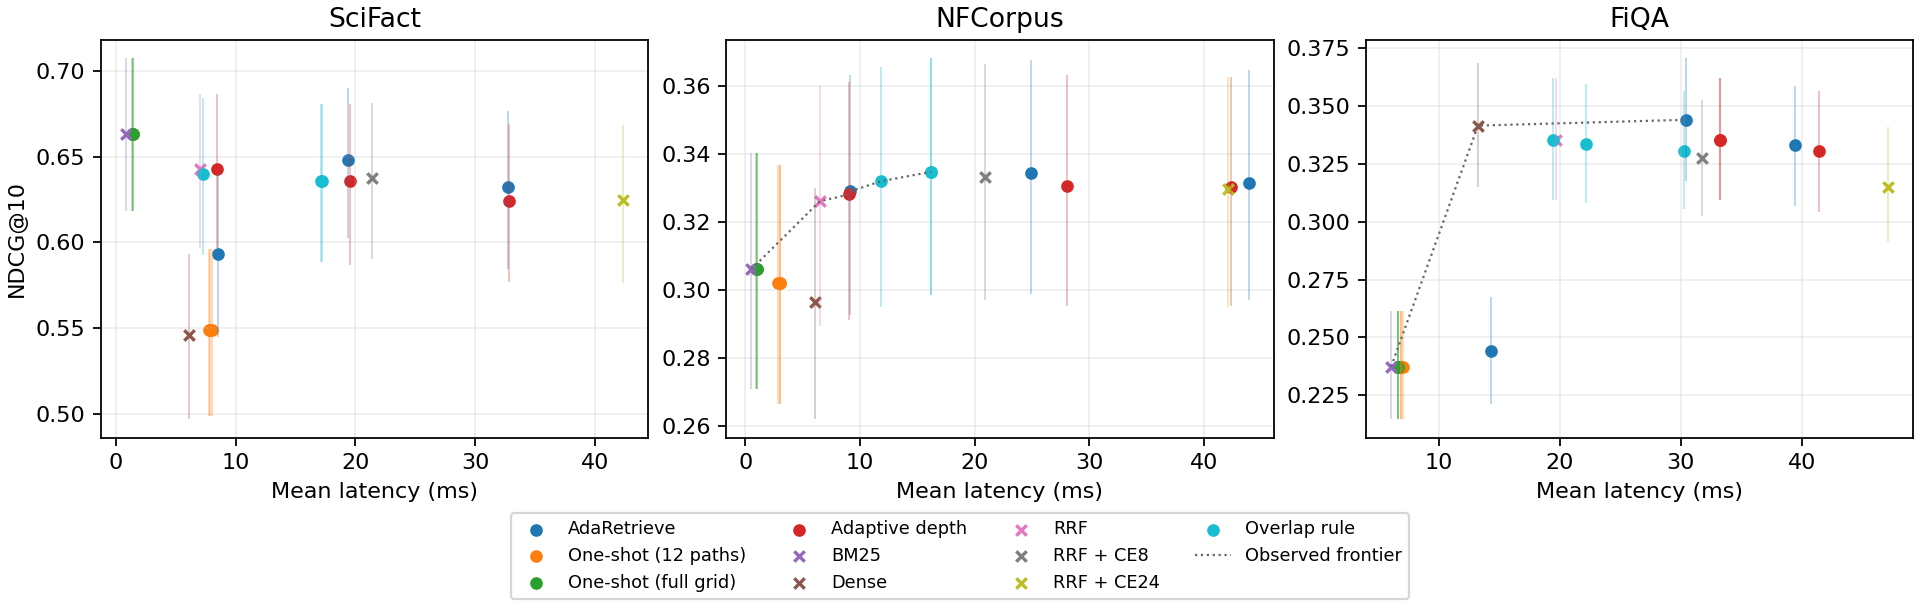
\includegraphics[width=\linewidth]{quality_latency.png}
\caption{Broad benchmark. Dotted segments join the observed nondominated quality--latency points across all ten main methods. Vertical bars are marginal 95\% query intervals for NDCG@10. On NFCorpus at the middle budget, the overlap rule (0.33484 in 16.19 ms) dominates the sequential point (0.33445 in 24.91 ms) by point estimate.}\label{fig:broad}
\end{figure}
\begin{figure}[h!]\centering
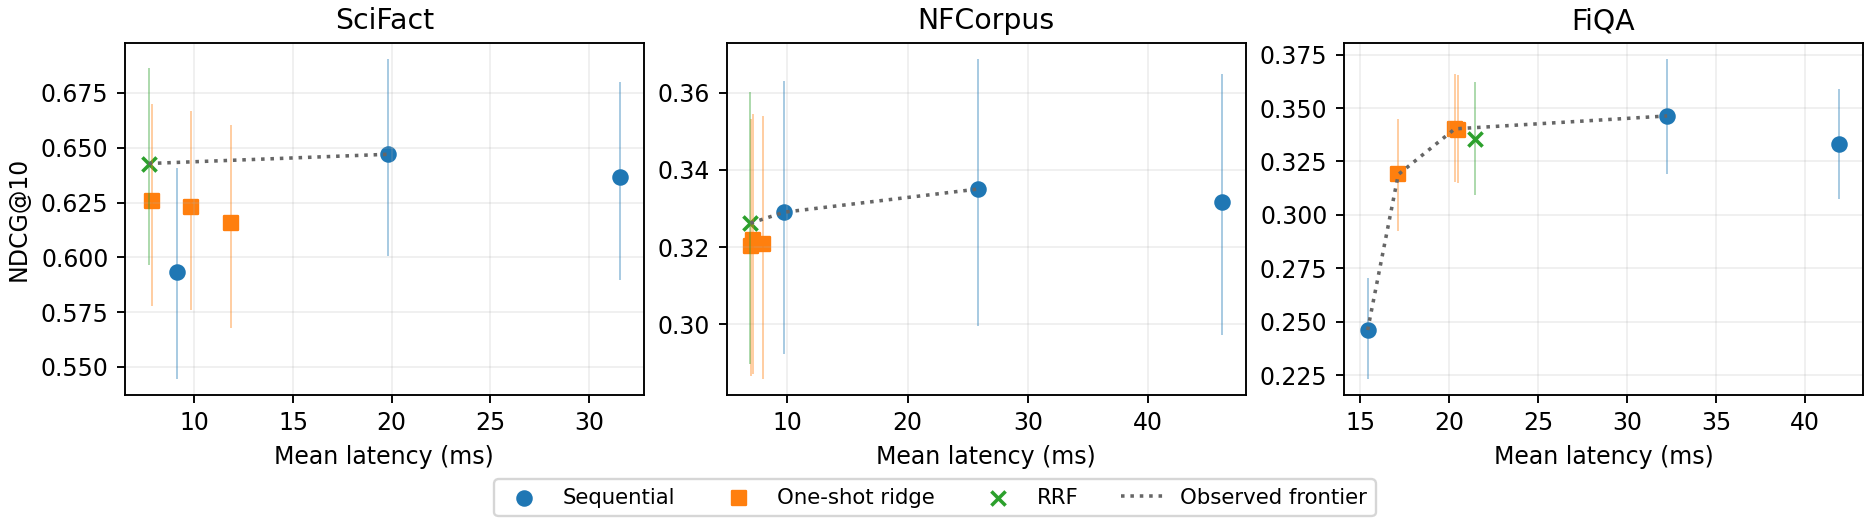
\includegraphics[width=\linewidth]{router_frontier.png}
\caption{First routing follow-up. Domain-level frontiers compare sequential control, one-shot routing and fixed RRF within this session. Budget guards can shorten the chosen path. Points represent rankings actually returned.}\label{fig:root}
\end{figure}
\clearpage
\section{Source confirmation and sensitivity}
On source-training queries that request both lexical depths, BM25 reuse reduces the median combined time from 1.384 to 0.715 ms on SciFact, from 0.532 to 0.275 ms on NFCorpus, and from 11.279 to 5.611 ms on FiQA. The rankings agree in the paired checks. Reuse also changes which actions fit the budget, so the end-to-end saving depends on the router.
\begin{table}[h!]\centering
\caption{Live source confirmation. Entries give the change from adding each component to its matched baseline. The same 144 distinct source queries occur in two folds each.}
\datatable{source}
\end{table}

\begin{table}[h!]\centering
\caption{Sequential ablations at the middle budget in the broad benchmark. The hard feasibility mask remains active when budget features are removed.}
\datatable{ablation}
\end{table}
\begin{figure}[h!]\centering
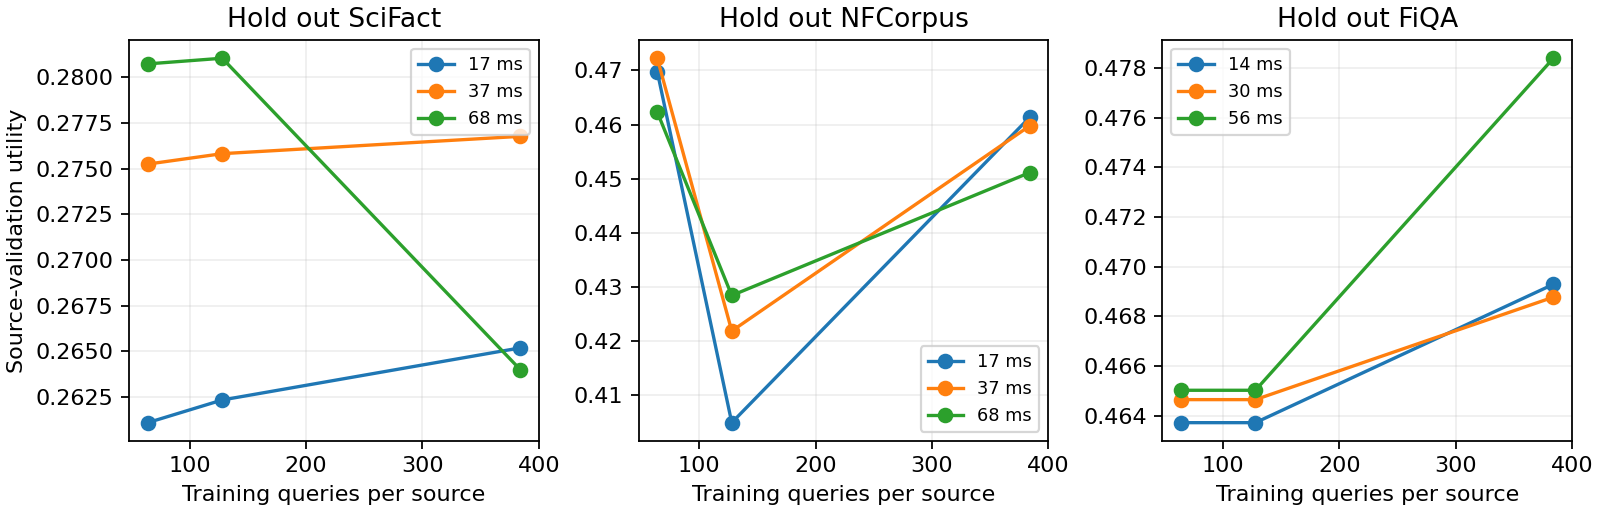
\includegraphics[width=\linewidth]{learning_curve.png}
\caption{Source-validation utility at increasing numbers of training queries per source. Curves use profiled costs. For NFCorpus held out, the middle-budget values at 64, 128 and 384 queries are 0.4723, 0.4218 and 0.4598. At 384, the middle-budget gaps to the source-validation oracle span 0.0827--0.1478 across folds.}\label{fig:learn}
\end{figure}
\end{document}
